% Basic stuff
\documentclass[a4paper,10pt]{article}
\usepackage[utf8]{inputenc}
\usepackage[nswissgerman]{babel}
\usepackage{scrextend}
\usepackage{lipsum}
\usepackage{amsmath}
\usepackage{gauss}
\usepackage{amssymb} % to import \leadsto

% 3 column landscape layout with fewer margins
\usepackage[landscape, left=0.75cm, top=1cm, right=0.75cm, bottom=1.5cm, footskip=15pt]{geometry}
\usepackage{flowfram}
\usepackage{floatrow}
\usepackage{amsmath}
\usepackage[inline]{enumitem}
\usepackage{pst-node}
\usepackage{auto-pst-pdf}
\usepackage{tikz-cd} 
\usepackage{multicol}


\changefontsizes[10pt]{8pt}
\ffvadjustfalse
\setlength{\columnsep}{1cm}
\Ncolumn{3}
\DeclareMathOperator{\Tr}{Tr}
\DeclareMathOperator{\Rank}{Rank}
\DeclareMathOperator{\Image}{Im}
\DeclareMathOperator{\Columnspace}{\mathcal{R}}
\DeclareMathOperator{\Nullspace}{\mathcal{N}}
\DeclareMathOperator{\Kernel}{Ker}
\DeclareMathOperator{\diag}{diag}
\DeclareMathOperator{\Span}{span}

% define nice looking boxes
\usepackage[most]{tcolorbox}

% a base set, that is then customised
\tcbset {
  base/.style={
    boxrule=0mm,
    leftrule=1mm,
    left=1.75mm,
    arc=0mm, 
    fonttitle=\bfseries, 
    colbacktitle=black!10!white, 
    coltitle=black, 
    toptitle=0.75mm, 
    bottomtitle=0.25mm,
    title={#1}
  }
}

\newcommand{\middot}{~\textperiodcentered~}
\newlist{rowlist}{enumerate*}{1}
\setlist[rowlist]{label={\textbf{\roman*}\text{: }}, afterlabel={}, itemjoin=\middot}

\makeatletter
\renewcommand*\env@matrix[1][*\c@MaxMatrixCols c]{%
  \hskip -\arraycolsep
  \let\@ifnextchar\new@ifnextchar
  \array{#1}}
\makeatother

\newcommand\undermat[2]{%
  \makebox[0pt][l]{$\smash{\underbrace{\phantom{%
    \begin{matrix}#2\end{matrix}}}_{\text{$#1$}}}$}#2}

\newcommand\overmat[2]{%
  \makebox[0pt][l]{$\smash{\overbrace{\phantom{%
    \begin{matrix}#2\end{matrix}}}^{\text{$#1$}}}$}#2}

\definecolor{brandblue}{rgb}{0.34, 0.7, 1}
\newtcolorbox{mainbox}[1]{
  colframe=brandblue, 
  base={#1}
}

\newtcolorbox{subbox}[1]{
  colframe=black!20!white,
  base={#1}
}

% Mathematical typesetting & symbols
\usepackage{amsthm, mathtools, amssymb} 
\usepackage{marvosym, wasysym}
\allowdisplaybreaks

% Tables
\usepackage{tabularx, multirow}
\usepackage{booktabs}

% Make enumerations more compact
\usepackage{enumitem}
\setitemize{itemsep=0.5pt}
\setenumerate{itemsep=0.75pt}

% To include sketches & PDFs
\usepackage{graphicx}

% For hyperlinks
\usepackage{hyperref}
\hypersetup{
  colorlinks=true
}

% Metadata
\title{Cheatsheet Lineare Algebra}
\author{Thomas Gassmann}
\date{August 2022}

% Math helper stuff
\def\limn{\lim_{n\to \infty}}
\def\limxo{\lim_{x\to 0}}
\def\limxi{\lim_{x\to\infty}}
\def\limxn{\lim_{x\to-\infty}}
\def\sumk{\sum_{k=1}^\infty}
\def\sumn{\sum_{n=0}^\infty}
\def\R{\mathbb{R}}
\def\C{\mathbb{C}}
\def\E{\mathbb{E}}
\def\K{\mathbb{K}}
\def\dx{\text{ d}x}

\newcommand{\overbar}[1]{\mkern 1.5mu\overline{\mkern-1.5mu#1\mkern-1.5mu}\mkern 1.5mu}

\begin{document}

\begin{center}
  Lizenziert unter CC BY-SA 4.0. Für Urheber, Quellen und Lizenzinformationen, siehe:\\
  \href{https://github.com/thomasgassmann/eth-summaries}{thomasgassmann/eth-summaries}
\end{center}

\section{Vorwissen}
\subsection{Komplexe Zahlen}
\begin{mainbox}{Definition}
Ein Ausdruck der Form $z = a + ib$, wobei $i^2 = -1$. $a = Re(z)$ ist der Realteil, $b = Im(z)$ ist der Imaginärteil.
\end{mainbox}

Addition erfolgt komponentenweise, Multiplikation erfolgt unter Annahme des Binomialgesetzes und $i^2 = -1$ (i.e. $z w = (a c - b d) + i (a d + b  c)$). Für Division gilt $\frac{z}{w} = \frac{c + id}{a + ib} = \frac{z\overbar{w}}{w\overbar{w}} = \frac{(ca + bd) + i(ad - cb)}{a^2 + b^2}$.\\
Die Norm ist definiert als $|z| = \sqrt{Re(z)^2 + Im(z)^2} = \sqrt{z \cdot \overbar{z}}$. Für $z = x + iy$ ist $\overbar{z} = x - iy$ konjugiert-komplex.

\begin{subbox}{}
$$z \overbar{z} = Re(z)^2 + Im(z)^2$$
\end{subbox}

Eine komplexe Zahl kann in Polarkoordinaten dargestellt werden. Es gilt $z = re^{i\phi} = r(\cos(\phi) + i\sin(\phi))$.
Radizieren: $\sqrt[n]{a} = z \iff a = z^n \iff |a| e^{i\alpha} = r^n e^{i\phi n}$ wobei $r = \sqrt[n]{|a|}$ und $\phi = \frac{\alpha + 2k\pi}{n}$.

\begin{mainbox}{Fundamentalsatz der Algebra}
  Sei $p(z) = a_n z^n + \cdots + a_0$ ein Polynom mit $a_n \neq 0$ und reellen oder komplexen Koeffizienten $a_i \in \mathbb{C}$. Dann hat $p(z)$ genau $n$ Nullstellen (mit ihren Vielfachen gezählt).
\end{mainbox}

Es gilt $\overbar{z \pm w} = \overbar{z} \pm \overbar{w}$, $\overbar{zw} = \overbar{z}\overbar{w}$, $\overbar{(\frac{z}{w})} = \frac{\overbar{z}}{\overbar{w}}$, $|\overbar{z}| = |z|$, $|z + w| \leq |z| + |w|$, $|zw| = |z| |w|$.

$$
\theta = \begin{cases}
  \arctan(\frac{y}{x}) \textbf{ if z on positive x-axis}\\
  \frac{\pi}{2} \textbf{ if }x=0, y > 0\\
  \pi + \arctan(\frac{y}{x}) \textbf{ if z on negative x-axis}\\
  \frac{3\pi}{2} \textbf{ if }x=0, y < 0
\end{cases}
$$

\subsection{Polynome}

Bei Polynomen mit reellen Nullstellen treten die Nullstellen als komplex konjugiertes Paar auf. Für Grad 2, verwende $z = \frac{-b \pm \sqrt{b^2 - 4ac}}{2a}$ um ein Polynom $p(z) = 0$ zu lösen. Für $a z^n + c = 0$, verwende $z = \sqrt[n]{-\frac{c}{a}}$.

Bei einem Polynom über $\mathbb{C}$ mit ungeradem Grad gibt es mindestens eine reelle Nullstelle.

\section{LGS / Gauss}

Ein homogenes LGS hat die Form $Ax = 0$.

\begin{enumerate}
  \item Wir können Zeilen austauschen, eine Zeile mit $a \in \mathbb{R}\setminus \{0\}$ multiplizieren und Zeilen voneinander subtrahieren bzw. addieren.
  \item Wir schreiben das lineare Gleichungssystem (LGS) in Matrixform.
  \item Wir transformieren das LGS in die Zeilenstufenform.
  \item Wir lösen das LGS von unten nach oben.
\end{enumerate}

\begin{center}
  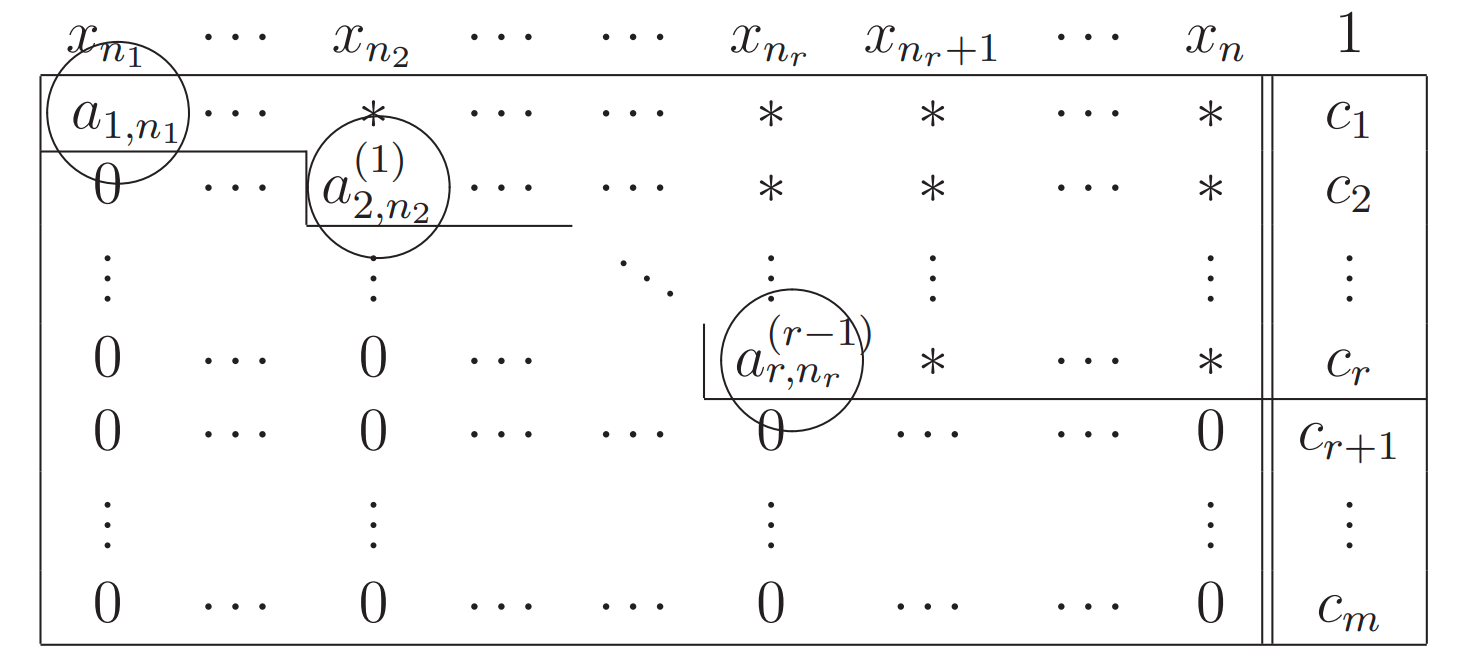
\includegraphics[width=\linewidth]{gauss.png}
\end{center}

\textbf{Verträglichkeitsbedingungen (VTB):} Falls die Verträglichkeitsbedingungen $c_{r+1} = \cdots = c_m = 0$ nicht erfüllt sind, so gibt es keine Lösung. Bei homogenen LGS sind die Verträglichkeitsbedingungen immer erfüllt. Nur wenn $r < n$ gibt es also nicht-triviale Lösungen.\\

\begin{subbox}{Lösungen}
  $Ax = b$ hat mindestens eine Lösung gdw. ($r = m$) oder ($r < m$ und VTB sind erfüllt). In diesem Fall gibt es 1 Lösung falls $r = n$, andernfalls eine $n - r$ Schar an Lösungen.
  \begin{itemize}
    \item $r = m$: $\begin{cases}
      r = m = n\text{: eindeutige Lösung, regulär}\\
      r < n\text{: }\infty\text{ Lösungen mit } n - r \text{ freien Variablen}
    \end{cases}$\\
    \item $r < m$: $\begin{cases}
      r = n\text{: eindeutige Lösung}\\
      r < n\text{: }\infty\text{ Lösungen mit } n - r \text{ freien Variablen}
    \end{cases}$
  \end{itemize}
\end{subbox}

Es gilt immer $r \leq \min(m, n)$.

\section{Matrizen \& Vektoren}

Eine $m \times n$ Matrix hat $m$ Zeilen und $n$ Spalten wobei das $i,j$ Element mit $a_{i,j}$ oder $(A)_{i,j}$ bezeichnet wird. Ein $m \times 1$ Vektor ist ein \textbf{Spaltenvektor} und ein $1 \times n$ Vektor ist ein \textbf{Zeilenvektor} (n-Tupel). Die Elemente $a_{jj}, j = 1,2,\cdots,\min(m,n)$ heissen \textbf{Diagonalelemente}. Für eine \textbf{Diagonalmatrix} $A$ gilt $(A)_{ij} = 0$ für $i = j$. Wir bezeichnen die Matrix dann durch die Elemente auf der Diagonale: $A = \diag(d_{11}, \cdots, d_{nn})$. Für eine \textbf{obere Dreiecksmatrix} gilt: $(R)_{ij} = 0$ für $i > j$. Für eine \textbf{untere Dreiecksmatrix} gilt: $(L)_{ij} = 0$ für $i < j$.

\begin{subbox}{Multiplikation}
  Für eine $m \times n$ Matrix $A$ und eine $n \times p$ Matrix $B$ gilt $(AB)_{ij} = \sumn a_{ik} b_{kj}$ wobei $AB$ eine $m \times p$ Matrix ist. Generell \textbf{nicht kommutativ}.
\end{subbox}

\begin{subbox}{Rechenregeln für Matrizen}
  \begin{rowlist}
    \item $(\alpha \beta)A = \alpha(\beta A)$
    \item $(\alpha A)B = \alpha(AB) = A(\alpha B)$
    \item $(\alpha + \beta)A = \alpha A + \beta A$
    \item $\alpha(A + B) = \alpha A + \alpha B$
    \item $A + B = B + A$
    \item $A + (B + C) = (A + B) + C$
    \item $(AB)C = A(BC)$
    \item $(A + B)C = AC + BC$
    \item $A(B + C) = AB + AC$
  \end{rowlist}
\end{subbox}

Eine \textbf{Linearkombination} der Vektoren $a_1, \cdots, a_n$ ist $\alpha_1 a_1 + \cdots + \alpha_n a_n$.\\
Falls $AB = 0$, so sind $A$ und $B$ \textbf{Nullteiler}.\\
\begin{subbox}{Transponierte Matrizen}
  \textbf{Transponiert}: $A^\top$ wird definiert als $(A^\top)_{ij} = (A)_{ji}$.\\
  \textbf{Hermitesch-transponiert}: $A^H = (\overbar{A})^\top = \overbar{A^\top}$.
\end{subbox}
Eine Matrix ist \textbf{symmetrisch} falls $A^\top = A$ und \textbf{hermitesch} falls $A^H = A$ (Diagonale somit reell). \textbf{Schiefsymmetrisch} ist sie falls $A^\top = -A$. 

Sind $A$ und $B$ hermitesche Matrizen, so ist $AB$ genau dann hermitesch falls $AB = BA$. $A^H A$ und $A A^H$ sind  immer hermitesch.

\begin{subbox}{Rechenregeln für hermitesche Matrizen}
  \begin{rowlist}
    \item $(A^\top)^\top = A$
    \item $(A^H)^H = A$
    \item $(\alpha A)^\top = \alpha A^\top$
    \item $(\alpha A)^H = \overbar{\alpha} A^H$
    \item $(A + B)^\top = A^\top + B^\top$
    \item $(A + B)^H = A^H + B^H$
    \item $(AB)^\top = B^\top A^\top$
    \item $(AB)^H = B^H A^H$
  \end{rowlist}
\end{subbox}

\begin{subbox}{Spalten- und Reihensichtweise}
  Ist $A = \begin{psmallmatrix}
    \underline{a_1} \\
    \cdots \\
    \underline{a_m}
  \end{psmallmatrix}$ eine $m \times n$ Matrix, $B = \begin{psmallmatrix}
    b_1 & b_2 & \cdots & b_p
  \end{psmallmatrix}$ eine $n \times p$ Matrix, dann gilt $AB = \begin{psmallmatrix}
    A b_1 & A b_2 & \cdots & A b_p
  \end{psmallmatrix} = \begin{psmallmatrix}
    \underline{a_1} B \\
    \cdots \\
    \underline{a_m} B
  \end{psmallmatrix}$.

  Ist umgekehrt $A = \begin{psmallmatrix}
    a_1 & a_2 & \cdots & a_n
  \end{psmallmatrix}$ eine $m \times n$ Matrix, $B = \begin{psmallmatrix}
    \underline{b_1} \\
    \cdots \\
    \underline{b_n}
  \end{psmallmatrix}$ eine $n \times p$ Matrix, dann gilt $AB = \sum_{i=1}^n a_i \underline{b_i}$.

\end{subbox}

Multipliziert man eine Diagonalmatrix von links, dann skaliert dies die Zeilen. Multipliziert man eine Diagonalmatrix von rechts, dann multipliziert dies die Spalten.

\begin{subbox}{Definite}
  Eine Matrix $A$ ist positiv-definit (positiv-semidefinit), falls $\forall x \in \E^n$, $x^H A x > 0$ ($\geq 0$).
\end{subbox}

Eine symmetrische Matrix $A$ ist genau dann positiv-definit (positiv-semidefinit) falls alle Eigenwerte strikt positiv (positiv) sind.

Um zu zeigen, dass eine Matrix $A$ indefinit ist, zeigt man, dass es ein $x$ mit $x^\top A x > 0$ und ein $y$ mit $y^\top A y < 0$ gibt. Es gilt $e_i^\top A e_j = a_{ij}$. Folglich ist $A$ indefinit, falls es auf der Diagonalen von $A$ verschiedene Vorzeichen gibt (vorrausgesetzt $\det(A) \neq 0$).

Das $\textbf{äussere Produkt}$ für zwei Vektoren $x$ und $y$ ist definiert als $xy^T$. Die \textbf{orthogonale Projektion} von $x$ auf $y$ ist $P_y x = \frac{1}{\lVert y \rVert^2} y y^H x$.

\subsection{Inverse}

Eine $n \times n$ Matrix ist $\textbf{invertierbar}$ wenn eine Matrix $A^{-1}$ existiert, so dass $A A^{-1} = I_n = A^{-1} A$. Die Inverse ist eindeutig bestimmt und existiert genau dann wenn $\Rank A = n$.

\begin{subbox}{Rechenregeln für Inverse}
  Sind $A, B$ regulär. Dann:

  \begin{itemize}
    \item $A^{-1}$ regulär und $(A^{-1})^{-1} = A$.
    \item $AB$ regulär und $(AB)^{-1} = B^{-1} A^{-1}$.
    \item $A^H$ regulär und $(A^H)^{-1} = (A^{-1})^H$.
  \end{itemize}
\end{subbox}

Die Inverse findet man durch Gauss-Jordan Elimination.

$$\begin{bmatrix*}
  A | I_n
\end{bmatrix*} \xRightarrow[\text{operationen}]{\text{Zeilen-}} \begin{bmatrix*}
  I_n | A^{-1}
\end{bmatrix*}$$

Für $A = \begin{psmallmatrix*}
  a & b \\
  c & d
\end{psmallmatrix*}$ und $\det(A) \neq 0$ (also $A$ invertierbar) gilt $A^{-1} = \frac{1}{ad - bc} \begin{psmallmatrix*}
  d & -b \\
  -c & a
\end{psmallmatrix*}$.

\subsection{Orthogonale und unitäre Matrizen}

Eine $n \times n$ Matrix heisst \textbf{unitär} falls $A^H A = I_n$. Eine unitäre Matrix heisst \textbf{orthogonal} falls $A^T A = I_n$. Es gilt $\det(A) = \pm 1$. Die Matrix ist genau dann unitär/orthogonal wenn alle Spalten orthonormal sind.

Für $A, B$ unitär (dasselbe für orthogonal) gilt:

\begin{itemize}
  \item $A$ regulär und $A^{-1} = A^H$
  \item $AA^H = I_n = A^H A$
  \item $A^{-1}$, $AB$ unitär
\end{itemize}

\subsection{Rotationsmatrizen}

Eine Rotationsmatrix $R$ ist eine unitäre Matrix. In 2D ist $R = \begin{psmallmatrix*}
  \cos \theta & -\sin \theta \\
  \sin \theta & \cos \theta
\end{psmallmatrix*}$. Verallgemeinert wird dies durch Givens-Rotationen. In 4D gilt bspw. $\begin{psmallmatrix}
  \cos \theta & 0 & -\sin \theta & 0 \\
  0 & 1 & 0 & 0 \\
  \sin \theta & 0 & \cos \theta & 0 \\
  0 & 0 & 0 & 1
\end{psmallmatrix}$.

\section{LR-Zerlegung}

Die \textbf{LR-Zerlegung} ist ein weiteres Verfahren zum lösen von LGS. Es ist besonders effektiv wenn wir mehrere LGS mit gleichem $A$ haben.

\begin{align*}
  & \begin{bmatrix}[ccc|ccc|ccc]
    \overmat{I}{1 & 0 & 0} & \overmat{A}{2 & 1 & 2} & \overmat{I}{1 & 0 & 0}\\
    0 & 1 & 0 & \textcolor{green}{1} & 2 & 3 & 0 & 1 & 0\\
    0 & 0 & 1 & \textcolor{blue}{2} & 2 & 2 & 0 & 0 & 1
  \end{bmatrix} \begin{matrix}
    \\
    \textcolor{green}{-\frac{1}{2}}\\
    \textcolor{blue}{-1}
  \end{matrix}\\
  \implies & \begin{bmatrix}[ccc|ccc|ccc]
    1 & 0 & 0 & 2 & 1 & 2 & 1 & 0 & 0\\
    0 & 1 & 0 & 0 & \frac{3}{2} & 2 & \textcolor{green}{\frac{1}{2}} & 1 & 0\\
    0 & 0 & 1 & 0 & \textcolor{cyan}{1} & 0 & \textcolor{blue}{1} & 0 & 1
  \end{bmatrix} \begin{matrix}
    \\
    \\
    \textcolor{cyan}{-\frac{2}{3}}
  \end{matrix}\\
  \implies & \begin{bmatrix}[ccc|ccc|ccc]
    1 & 0 & 0 & 2 & 1 & 2 & 1 & 0 & 0\\
    0 & 1 & 0 & 0 & \frac{3}{2} & 2 & \textcolor{green}{\frac{1}{2}} & 1 & 0\\
    \undermat{P}{0 & 0 & 1} & \undermat{R}{0 & 0 & -\frac{4}{3}} & \undermat{L}{\textcolor{blue}{1} & \textcolor{cyan}{\frac{2}{3}} & 1}
  \end{bmatrix}
\end{align*}\\

Wenn wir Zeilen vertauschen, dann ändert sich $P$. Haben wir eine LR-Zerlegung von $A$ können wir $Ax = b$ effizienter lösen. Zuerst lösen wir dazu $PA = LR$ und lösen $Lc = Pb$ nach $c$. Dann lösen wir $Rx = c$ nach $x$.

\section{Vektorräume}

\begin{mainbox}{}
  Eine Vektorraum $V$ über $\K$ ist eine nichtleere Menge auf dere eine Vektoraddition und Skalarmultiplikation definiert sind.
  \begin{enumerate}[label=V\arabic*]
    \item $x + y = y + x$
    \item $(x + y) + z = x + (y + z)$
    \item $\exists 0 \in V: x + 0 = x$ ($\forall x \in V$)
    \item $\forall x \in V$ existiert $-x$: $x + (-x) = 0$
    \item $\alpha(x + y) = \alpha x + \alpha y$
    \item $(\alpha + \beta)x = \alpha x + \beta x$
    \item $(\alpha \beta)x = \alpha (\beta x)$
    \item $\exists 1 \in \K$ so dass $\forall x \in V: 1x = x$
    \end{enumerate}
\end{mainbox}

\begin{rowlist}
  \item $0x = 0$
  \item $\alpha 0 = 0$
  \item $\alpha x = 0 \implies x = 0 \vee \alpha = 0$
  \item $(-\alpha)x = \alpha (-x) = -(\alpha x)$
\end{rowlist}

\subsection{Unterräume}

Ein Unterraum $U$ ist eine nichtleere Teilmenge von $V$ der abgeschlossen bzgl. Addition und Multiplikation ist. $U$ beinhaltet immer den Nullvektor. Jeder Unterraum ist ein Vektorraum. 

\begin{subbox}{Lineare Hülle}
  Die Menge der Linearkombinationen der Vektoren $v_1, \cdots, v_n$ ist der Unterraum aufgespannt durch diese Vektoren. Man bezeichnet ihn mit $\Span \{ v_1, \cdots, v_n \}$.
\end{subbox}

Falls $\Span {v_1, \cdots, v_n} = V$, dann sind $v_1, \cdots, v_n$ ein \textbf{Erzeugendensystem} von $V$.

Um zu zeigen dass $U \subseteq V$ ein Unterraum von $V$ ist zeigt man folgende Dinge:
\begin{itemize}
  \item $0_V \in U$
  \item $\forall x, y \in U$ gilt $x + y \in U$
  \item $\forall x \in U, \forall \alpha \in \K$ gilt $\alpha x \in U$
\end{itemize}

\subsection{Lineare Abhängigkeit, Basen und Dimensionen}

\begin{mainbox}{Lineare Unabhängigkeit}
  Vektoren $v_1, \cdots, v_n$ sind linear unabhängig genau dann wenn:
  $$\sum_{k=1}^n \alpha_k v_k = 0 \iff \alpha_1 = \cdots = \alpha_n = 0$$
  Andernfalls sind die Vektoren linear abhängig.
\end{mainbox}

\begin{mainbox}{Basis}
  Ein Erzeugendensystem $v_1, \cdots, v_n$ von $V$ ist eine Basis von $V$ genau dann wenn $v_1, \cdots, v_n$ linear unabhängig sind.
\end{mainbox}

Jede Menge $\{v_1, \cdots, v_m\} \subseteq V$ mit $\dim V < m$ ist linear abhängig. In jedem endlichen Vektorraum $V$ mit $\dim V = n$ ist eine Menge von $n$ linear unabhängigen Vektoren eine Basis.

Die Koeffizienten $\xi = (\xi_1, \cdots, \xi_n)^\top$ sind \textbf{Koordinaten} von $x$ bzgl. einer Basis $\mathcal{B}$ falls $x = \sum_{i=1}^n \xi_i b_i$ gilt. Die Summe wird Koordinatendarstellung genannt.

Zwei Unterräume $U, W \subseteq V$ heissen \textbf{komplementär} falls jedes $x \in V$ eine eindeutige Darstellung $x = u + w$ mit $u \in U$ und $w \in W$ hat ($V$ ist dann direkte Summe von $U$ und $W$). Man schreibt $V = U \oplus W$. Falls zwei Unterräume komplementär sind, folgt $U \cap W = \{0_V\}$.

Falls  $f: U \rightarrow V$ und $g: V \rightarrow W$ lineare Abbildungen zwischen Vektorräumen sind so dass $ g \circ f$ ein Isomorphismus ist, dann gilt $V = \operatorname{Im}f \oplus \operatorname{Ker} g$.

\subsection{Basiswechsel und Koordinatentransformation}

Wenn wir von einer alten Basis $\mathcal{B}$ zu einer neuen Basis $\mathcal{B}'$ wechseln, können wir die neue Basis mit der alten darstellen. Es gilt dann $b_k' = \sum_{i=1}^n \tau_{ik} b_i$ mit der \textbf{Basiswechselmatrix} $T = (\tau_{ik})$.

Es gilt $\xi = T \xi'$ sowie $\xi' = T^{-1} \xi$, da $T$ regulär ist. Dabei sind $\xi'$ die Koordinaten in der Basis $\mathcal{B}'$ und $\xi$ sind die Koordinaten in der Basis $\mathcal{B}$. Es gilt dann $\mathcal{B}' = \mathcal{B} T$.

\section{Lineare Abbildungen}

Eine Abbildung $F: V \mapsto W$ ist linear, wenn $F(v + w) = F(v) + F(w)$ sowie $F(\alpha v) = \alpha F(v)$ für alle $v, w \in V$ und $\alpha \in \K$ gilt. Einfacher ausgedrückt ist $F$ linear falls $F(\alpha v + w) = \alpha F(v) + F(w)$. 

Für eine Funktion $F: X \mapsto Y$ gilt:
\begin{itemize}
  \item \textbf{injektiv:} $\forall x, x' \in X$ $f(x) = f(x') \implies x = x'$
  \item \textbf{surjektiv:} $\forall y \in Y$ gibt es $x \in X$ mit $f(x) = y$
  \item \textbf{bijektiv:} injektiv und surjektiv, $F^{-1}$ existiert
\end{itemize}

Sei $F: X \mapsto Y$ eine lineare Abbildung ist wobei $\Span \{ b_1, \cdots, b_n \} = X$ und $\Span \{ c_1, \cdots, c_m \} = Y$ Basen sind.

Dann lässt sich $F(b_l) = \sum_{k=1}^m a_{kl} c_k$ schreiben. Die Matrix $A^{m \times n}$ mit Elementen $a_{kl}$ heisst die Abbildungsmatrix bezüglich $X, Y$.

Ist $F$ bijektiv ist es ein Isomorphismus, ist zusätzlich $X = Y$ so ist $F$ ein Automorphismus. Wenn $F$ ein Isomorphismus ist, existiert ein Isomorphismus $F^{-1}$.

\subsection{Kern, Bild und Rang}

Sei $F: X \mapsto Y$ eine lineare Abbildung.

\begin{mainbox}{Kern und Bild}

  Wir definieren den \textbf{Kern} als $\Kernel F := \{x \in X | F(x) = 0\}$. Der Kern ist ein Unterraum von $X$ und $F$ ist injektiv genau dann wenn $\Kernel F = \{0\}$

  Wir definieren das \textbf{Bild} als $\Image F := \{F(x) | x \in X\}$. Das Bild ist ein Unterraum von $Y$ und $F$ ist surjektiv genau dann wenn $\Image F = Y$.
\end{mainbox}

Es gilt $\Rank F := \dim \Image F$.

\begin{mainbox}{Rangsatz}
  $$\dim X - \dim \Kernel F = \dim \Image F = \Rank F$$
\end{mainbox}

\begin{subbox}{Foldergungen des Rangsatzes}
  Seien $F: X \mapsto Y, G: Y \mapsto Z$ lineare Abbildungen:
  \begin{itemize}
    \item $F$ injektiv $\iff$ $\Rank F = \dim X$
    \item $F$ surjektiv $\iff$ $\Rank F = \dim Y$
    \item $F$ bijektiv $\iff$ $\Rank F = \dim X = \dim Y$
    \item $\Rank G \circ F \leq \min(\Rank F, \Rank G)$
    \item $G$ injektiv $\implies$ $\Rank GF = \Rank F$
    \item $F$ surjektiv $\implies$ $\Rank GF = \Rank G$
  \end{itemize}
\end{subbox}

\subsection{Matrizen als lineare Abbildungen}

Sei $A \in \E^{m \times n}$. Der \textbf{Spaltenraum} von $A$ ist der Unterraum $\Columnspace(A) = \Image A = \Span \{ a_1, \cdots, a_n \} \subseteq \E^m$. Der \textbf{Nullraum} von $A$ ist der Unterraum $\Nullspace(A) = \Kernel A$.


\begin{subbox}{Rangsatz für Matrizen}
  Sei $r := \Rank A = \dim \Image A$. Dann ist $n - \dim \Kernel A = r$ und $r$ entspricht der Anzahl Pivotelemente in REF. Zusätzlich:
  
  $$\Rank A^T = \Rank A^H = \Rank A$$
\end{subbox}

Somit gilt für Matrizen $A \in \E^{m \times n}$ und $B \in \E^{p \times n}$ auch:

\begin{itemize}
  \item $\Rank BA \leq \min(\Rank A, \Rank B)$
  \item $\Rank B = m \leq p \implies \Rank BA = \Rank A$
  \item $\Rank A = m \leq n \implies \Rank BA = \Rank B$
\end{itemize}

Für quadratische Matrizen $A \in \E^{n \times n}$ sind also folgende Aussagen äquivalent:

\begin{rowlist}
  \item $A$ ist regulär
  \item $\Rank A = n$
  \item Spalten (und Zeilen) sind linear unabhängig
  \item $\Kernel A = \{0\}$
  \item $\Image A = \E^n$
\end{rowlist}

Falls $x_0$ eine Lösung für $Ax = b$ ist, so ist die Lösungsmenge $\mathcal{L}_b = x_0 + \Kernel A$ ein affiner Unterraum.

\subsection{Zusammenfassende Eigenschaften von $A$}

Sei $A \in M^{m \times n}$ mit $r := \Rank A$:

\begin{rowlist}
  \item $\dim \Image A = \dim \Image A^H = r$
  \item $\dim \Kernel A = n - r$
  \item $\dim \Kernel A^H = m - r$
\end{rowlist}

\begin{align*}
  r = n & \Leftrightarrow \Kernel A = \{ 0 \} & r = m & \Leftrightarrow \Kernel A^H = \{ 0 \} \\
  & \Leftrightarrow \text{Spalten von $A$ l.u.} & & \Leftrightarrow \text{Spalten von $A$ erzeugend}\\
  & \Leftrightarrow \text{Zeilen von $A$ erzeugend} & & \Leftrightarrow \text{Zeilen von $A$ l.u.}\\
  & \Leftrightarrow A \text{ injektiv} & & \Leftrightarrow A \text{ surjektiv}
\end{align*}

\begin{subbox}{Basis für $\Image A$ und $\Kernel A$ finden}
  Zuerst bringt man $A$ auf Zeilenstufenform.
  \begin{itemize}
    \item \textbf{Basis für $\Image A$}: Die Spalten in der \textit{originalen} Matrix welche den Pivotspalten in der Zeilenstufenform entsprechen sind Basisvektoren für $\Image A$.
    \item \textbf{Basis für $\Kernel A$}: Zuerst parameterisiert man die freien Variablen und findet dann die Lösungesmenge $\mathcal{L}_0$ von $Ax = 0$. Die Zeile $i$ des Lösungsvektors enthält dann den Wert der $i$-ten Variable. Man wählt dann die Koeffizienten der freien Variablen entsprechend um Basisvektoren zu finden (e.g. man setzt einen der Koeffizienten auf $1$ und alle anderen auf $0$ pro Basisvektor). 
  \end{itemize}
\end{subbox}

\subsection{Abbildungen von Koordinatentransformation}



\begin{multicols}{2}
  \begin{tikzcd}
    x \in X \arrow{r}{F} \arrow[shift left=1]{d}{\kappa_X}  & y \in Y \arrow[shift left=1]{d}{\kappa_Y} \\
    \xi \in \E^n \arrow{r}{A} \arrow[shift left=1]{u}{\kappa_X^{-1}} \arrow[shift left=1]{d}{T^{-1}} & \eta \in \E^m \arrow[shift left=1]{u}{\kappa_Y^{-1}} \arrow[shift left=1]{d}{S^{-1}} \\
    \xi' \in \E^n \arrow[shift left=1]{u}{T} \arrow{r}{B} & \eta' \in \E^m \arrow[shift left=1]{u}{S}
  \end{tikzcd}
  \begin{subbox}{}
    Es gilt:
    \begin{itemize}
      \item $A = SBT^{-1}$
      \item $B = S^{-1}AT$
    \end{itemize}
  \end{subbox}
\end{multicols}

Ist $F$ $\Rank F = r$, so besitzt $F$ bzgl. geeigneten Basen $X, Y$ die Abbildungsmatrix: 
\[
  \left[\begin{array}{ c | c }
    I_r & 0 \\
    \hline
    0 & 0
  \end{array}\right]
\]

\section{Vektorräume mit Skalarprodukt}

\begin{subbox}{Norm}
  Norm in Vektorraum $V$ über $\mathbb{E}$ ist eine Funktion $\lVert \cdot \rVert: V \mapsto \mathbb{R}$ mit:
  \begin{itemize}
    \item positiv definit: $\forall x \in V$, $\lVert x \rVert \geq 0$ und $\lVert x \rVert = 0 \iff x = 0$
    \item homogen: $\lVert \alpha x \rVert = \lvert \alpha \rvert \cdot \lVert x \rVert$ $\forall x \in V, \forall \alpha \in \mathbb{E}$
    \item Dreiecksungleichung: $\lVert x + y \rVert \leq \lVert x \rVert + \lVert y \rVert$ $\forall x, y \in V$
  \end{itemize}
  Ein Vektorraum mit einer Norm heisst normierter Vektorraum.
\end{subbox}

\begin{subbox}{Skalarprodukt}
  Skalarprodukt in einem Vektorraum $V$ über $\mathbb{E}$ ist eine Funktion $\langle \cdot, \cdot \rangle : V \times V \mapsto \mathbb{E}$ mit folgenden Eigenschaften:
  \begin{itemize}
    \item Linear im zweiten Faktor: $\langle x, y + z \rangle = \langle x, y \rangle + \langle x, z \rangle$ und $\langle x, \alpha y \rangle = \alpha \langle x, y \rangle$. Für reelle Skalare auch linear im ersten Faktor.
    \item  Symmetrisch wenn $\mathbb{E} = \mathbb{R}$ und hermitesch wenn $\mathbb{E} = \mathbb{C}$: $\langle x, y \rangle = \overbar{\langle y, x \rangle}$
    \item Positiv definit: $\forall x \in V$, $\langle x, x \rangle \in \mathbb{R}$ (auch für komplexe Vektorräume!), $\langle x, x \rangle \geq 0$, $\langle x, x \rangle = 0 \iff x = 0$
  \end{itemize}
  Falls $\mathbb{E} = \mathbb{C}$, nennt man $V$ auch einen unitären Vektorraum, für $\mathbb{E} = \mathbb{R}$ auch euklidischer oder orthogonaler Vektorraum. Für ein Skalarprodukt definiert man die induzierte Norm als $\lVert x \rVert = \sqrt[]{\langle x, x \rangle}$.
\end{subbox}

\begin{subbox}{Euklidischer Raum}
  Das euklidische Skalarprodukt ist definiert als: $$\langle x, y \rangle := x^H y$$
  Die euklidische 2-Norm ist entsprechend definiert als: $$\lVert x \rVert_2 = \sqrt[]{x^\top x}$$
\end{subbox}

Die $p$-Norm ist definiert als $\lVert x \rVert_p = (|x_1|^p + \cdots + |x_n|^p)^{\frac{1}{p}}$.

\begin{subbox}{Skalarprodukte über $\R^n$}
  $\langle x, y \rangle$ ist ein Skalarprodukt über $\R^n$ genau dann wenn $\langle x, y \rangle = x^\top A y$ wobei $A$ eine hermitesche Matrix mit strikt positiven Eigenwerten ist (positiv-definit).
\end{subbox}

\begin{mainbox}{Cauchy-Schwarz}
  Sei $V$ ein Vektorraum über $\mathbb{E}$ mit Skalarprodukt.
  $$| \langle x, y \rangle | ^2 \leq \langle x, x \rangle \langle y, y \rangle = \lVert x \rVert^2 \lVert y \rVert^2$$
  Das Gleichheitszeichen gilt genau dann wenn $x$ und $y$ linear abhängig sind.
\end{mainbox}

\begin{subbox}{Winkel}
  Seien $x, y, \in V$. Der Winkel zwischen $x$ und $y$ ist gegeben als:
  $$\varphi := \arccos \frac{Re \langle x, y \rangle}{\lVert x \rVert \lVert y \rVert}$$
\end{subbox}

Zwei Vektoren sind \textbf{orthogonal}, falls $\langle x, y \rangle = 0$ ($x \perp y$). Zwei Teilmengen sind orthogonal, wenn $\forall x \in M, \forall y \in N$ gilt: $\langle x, y \rangle = 0$ ($M \perp N$).

Eine Basis ist \textbf{orthogonal} wenn $\langle b_l, b_k \rangle = 0$ für alle $b_l \neq b_k$. Gilt zusätzlich $\lVert b_i \rVert = 1$ $\forall i$ ist sie \textbf{orthonormal}.

\begin{subbox}{Pythagoras}
  Falls $x \perp y$, so folgt $\lVert x \pm y \rVert^2 = \lVert x \rVert^2 + \lVert y \rVert^2$.
\end{subbox}

Eine Menge von paarweise orthogonalen Vektoren ist linear unabhängig wenn alle Vektoren ungleich null sind.

Für eine Orthonormalbasis $\{b_1, \cdots, b_n\}$ und $x \in V$ gilt $x = \sum_{k=1}^n \langle b_k, x \rangle b_k$.

\begin{mainbox}{Parsevalsche Formel}
  Seien $x, y \in V$, $\{ b_1, \cdots, b_n \}$ eine Orthonormalbasis, so dass $\xi_k := \langle b_k, x \rangle_V$ und $\eta_k := \langle b_k, y \rangle_V$. Für $k = 1, \cdots, n$ sind $\xi_k$ und $\eta_k$ die Koordinatenvektoren. 

  $$\langle x, y \rangle_V = \Sigma_{k=1}^n \overbar{\xi_k} \eta_k = \xi^H \eta = \langle \xi, \eta \rangle_{\E^n}$$

  \begin{rowlist}
    \item $\lVert x \rVert_V = \lVert \xi \rVert_{\E^n}$
    \item $\angle (x,y)_V = \angle (\xi, \eta)_{\E^n}$
    \item $x \perp y \iff \xi \perp \eta$
  \end{rowlist}
\end{mainbox}

\subsection{Gram-Schmidt-Orthonormalisierungsverfahren}

\begin{mainbox}{Algorithmus}
  Sei $\{a_1, \cdots, a_n\}$ eine Menge linear unabhängiger Vektoren. Wir definieren rekursiv:
  \begin{itemize}
    \item $b_1 := \frac{a_1}{\lVert a_1 \rVert}$
    \item $\widetilde{b_k} := a_k - \sum_{j=1}^{k-1} \langle b_j, a_k \rangle b_j$
    \item $b_k := \frac{\widetilde{b_k}}{\lVert \widetilde{b_k} \rVert}$
  \end{itemize}

  Nach $k$ Schritten sind $\{b_1, \cdots b_k\}$ paarweise orthonormal. Wenn $\{a_1, \cdots, a_n\}$ eine Basis von $V$ ist, ist $\{b_1, \cdots b_n\}$ auch eine. Jeder endlichdimensionale Vektorraum hat eine Orthonormalbasis.
\end{mainbox}
 
\begin{subbox}{Orthogonales Komplement}
  Für einen Unterraum $U$ von $V$ ist $U^\bot := \{ y \in V | \{y\} \bot U \}$ das orthogonale Komplement. $U$ und $U^\bot$ sind komplementäre Unterräume in direkter Summe zu $V$.
\end{subbox}

\begin{mainbox}{Fundamentale Unterräume einer Matrix}
  Sei $A \in \E^{m \times n}$ mit $r := \Rank A$.
  \begin{align*}
    & \Nullspace(A) = \Columnspace(A^H)^\perp \subseteq \E^n & & \Nullspace(A) \oplus \Columnspace(A^H) = \E^n\\
    & \Nullspace(A^H) = \Columnspace(A)^\perp \subseteq \E^m & & \Nullspace(A^H) \oplus \Columnspace(A) = \E^m\\
    & \dim \Columnspace(A) = r & & \dim \Nullspace(A) = n - r\\
    & \dim \Columnspace(A^H) = r & & \dim \Nullspace(A^H) = m - r
  \end{align*}
\end{mainbox}

\subsection{Basiswechsel und Koordinatentransformation von Orthonormalbasen}


\section{Determinanten}

TODO: Satz 8.12
TODO: positiv definit von ana2 summary, all eigenvlaues positive, TODO: 

\section{Eigenwerte und Eigenvektoren}

\begin{subbox}{Eigenschaften von Eigenwerten und Eigenvektoren}
  Für jede Matrix $A \in \mathbb{E}^{n \times n}$ gilt:
  $$\det(A) = \prod_{i=1}^{n} \lambda_i$$
  $$\Tr(A) = \Sigma_{i=1}^n \lambda_i$$
\end{subbox}

\section{Spektral- und Eigenwertzerlegung}

Wenn $\E^n$ eine Basis aus Eigenvektoren von $A \in \E^{n \times n}$ besitzt, so ist $A$ ähnlich zu einer Diagonalmatrix $\Lambda$.

$$A \underbrace{\begin{bsmallmatrix}
  \vert & \vert & \vert \\
  v_1   & \cdots & v_n   \\
  \vert & \vert & \vert
\end{bsmallmatrix}}_V = \underbrace{\begin{bsmallmatrix}
  \vert & \vert & \vert \\
  v_1   & \cdots & v_n   \\
  \vert & \vert & \vert
\end{bsmallmatrix}}_V \underbrace{\begin{bsmallmatrix}
  \lambda_1 & \cdots & 0 \\
  \vdots & \ddots & \vdots \\
  0 & \cdots & \lambda_n
\end{bsmallmatrix}}_\Lambda$$ $$ A = V \Lambda V^{-1}, Av_j = v_j \lambda_j, j = 1, \cdots, n$$

$A$ wird durch $V$ diagonalisiert.

\begin{subbox}{Normale Matrizen}
  Eine Matrix $A \in \E^{n \times n}$ ist normal, falls $A^H A = A A^H$. $A$ ist genau dann diagonalisierbar durch eine unitäre Matrix über $\C$ falls $A$ normal ist. 
\end{subbox}

\section{Singulärwärtszerlegung}

Die Singulärwärtszerlegung existiert für jede Matrix $A \in \E^{m \times n}$. $A^H A$ ist immer hermitesch und positiv-definit. Es existiert also eine Spektralzerlegung:

\begin{align*}
  A^H A V = V \Lambda & \xRightarrow[\text{Umordnung}]{\lambda = \sigma^2} & A^H A V_r = V_r \Sigma_r^2\\
  & \implies & V_r^H A^H A V_r = \Sigma_r^2\\
  & \implies & \underbrace{(\Sigma_r^{-1} V_r^H A^H)}_{U_r^{-1}} \underbrace{(A V_r \Sigma_r^{-1})}_{U_r} = I\\
\end{align*}

$U_r$ kann zu einer unitären Matrix $U$ ergänzt werden. $U, V$ sind unitär, $\Sigma$ ist nicht-negativ und diagonal mit $\sigma_1 \geq \cdots \sigma_r > \sigma_{r+1} = \cdots = \sigma_n = 0$ wobei $r = \Rank A = \Rank A^H A$. $V$ diagonalisiert $A^H A$, $U$ diagonalisiert $A A^H$.

$$A = U \Sigma V^H, AA^H = U \Sigma_m^2 U^H, A^H A = V \Sigma_n^2 V^H$$

Ausserdem gilt $A^H = V \Sigma^T U^H$ und falls $A$ invertierbar ist $A^{-1} = V \Sigma^{-1} U^H$.

\begin{itemize}
  \item $\{u_1, \cdots, u_r\}$: Basis von $\Image A = \Columnspace(A)$
  \item $\{u_{r+1}, \cdots, u_m\}$: Basis von $\Kernel A^H = \Nullspace(A^H)$
  \item $\{v_1, \cdots, v_r\}$: Basis von $\Image A^H = \Columnspace(A^H)$
  \item $\{v_{r+1}, \cdots, v_m\}$: Basis von $\Kernel A = \Nullspace(A)$
\end{itemize}

TODO: last chapoter, cahpter 10 missing in summary danny

\section{Tabellen}

\begin{mainbox}{Wichtige Werte}
  \begin{center} 
   \begin{tabular}{c|cccccc}
    deg & 0° & 30° & 45° & 60° & 90° & 180° \\
    \midrule
    rad & 0 & $\frac{\pi}{6}$ & $\frac{\pi}{4}$ & $\frac{\pi}{3}$ & $\frac{\pi}{2}$ & $\pi$ \\
    cos & 1 & $\frac{\sqrt{3}}{2}$ & $\frac{\sqrt{2}}{2}$ & $\frac{1}{2}$ & 0 & -1 \\
    sin & 0 & $\frac{1}{2}$ & $\frac{\sqrt{2}}{2}$ & $\frac{\sqrt{3}}{2}$ & 1 & 0 \\
    tan & 0 & $\frac{1}{\sqrt{3}}$ & 1 & $\sqrt{3}$ & $+\infty$ & 0 \\
   \end{tabular}
  \end{center}
\end{mainbox}

\begin{center}
  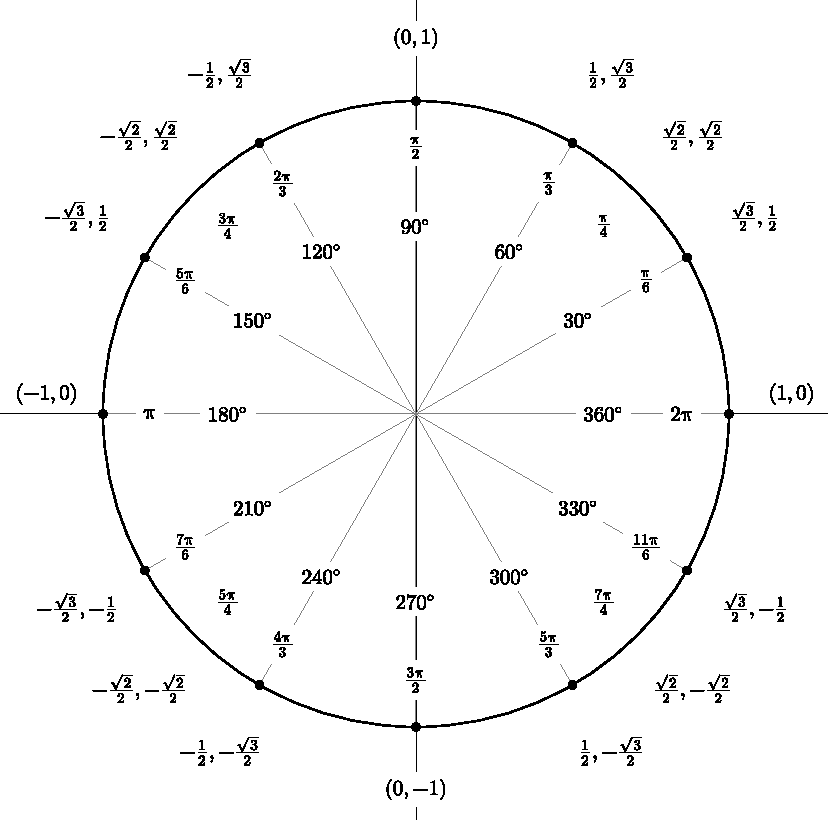
\includegraphics[width=\linewidth]{degrees_circle.pdf}
\end{center}

\end{document}
